\chapter{Progettazione concettuale}

    \section{Introduzione alla Progettazione}
    
    In questa sezione verrà illustrata la progettazione concettuale del lavoro svolto in UML. Verrà poi svolta e illustrata una ristrutturazione che verrà analizzata nella sezione "Ristrutturazione", andando a descrivere le giustificazioni dietro le scelte applicate, che fungeranno da fondamenta per il Class Diagram Ristrutturato.
        
    \section{Class Diagram e Ristrutturazione}
        \begin{figure}[h]
           \centering
           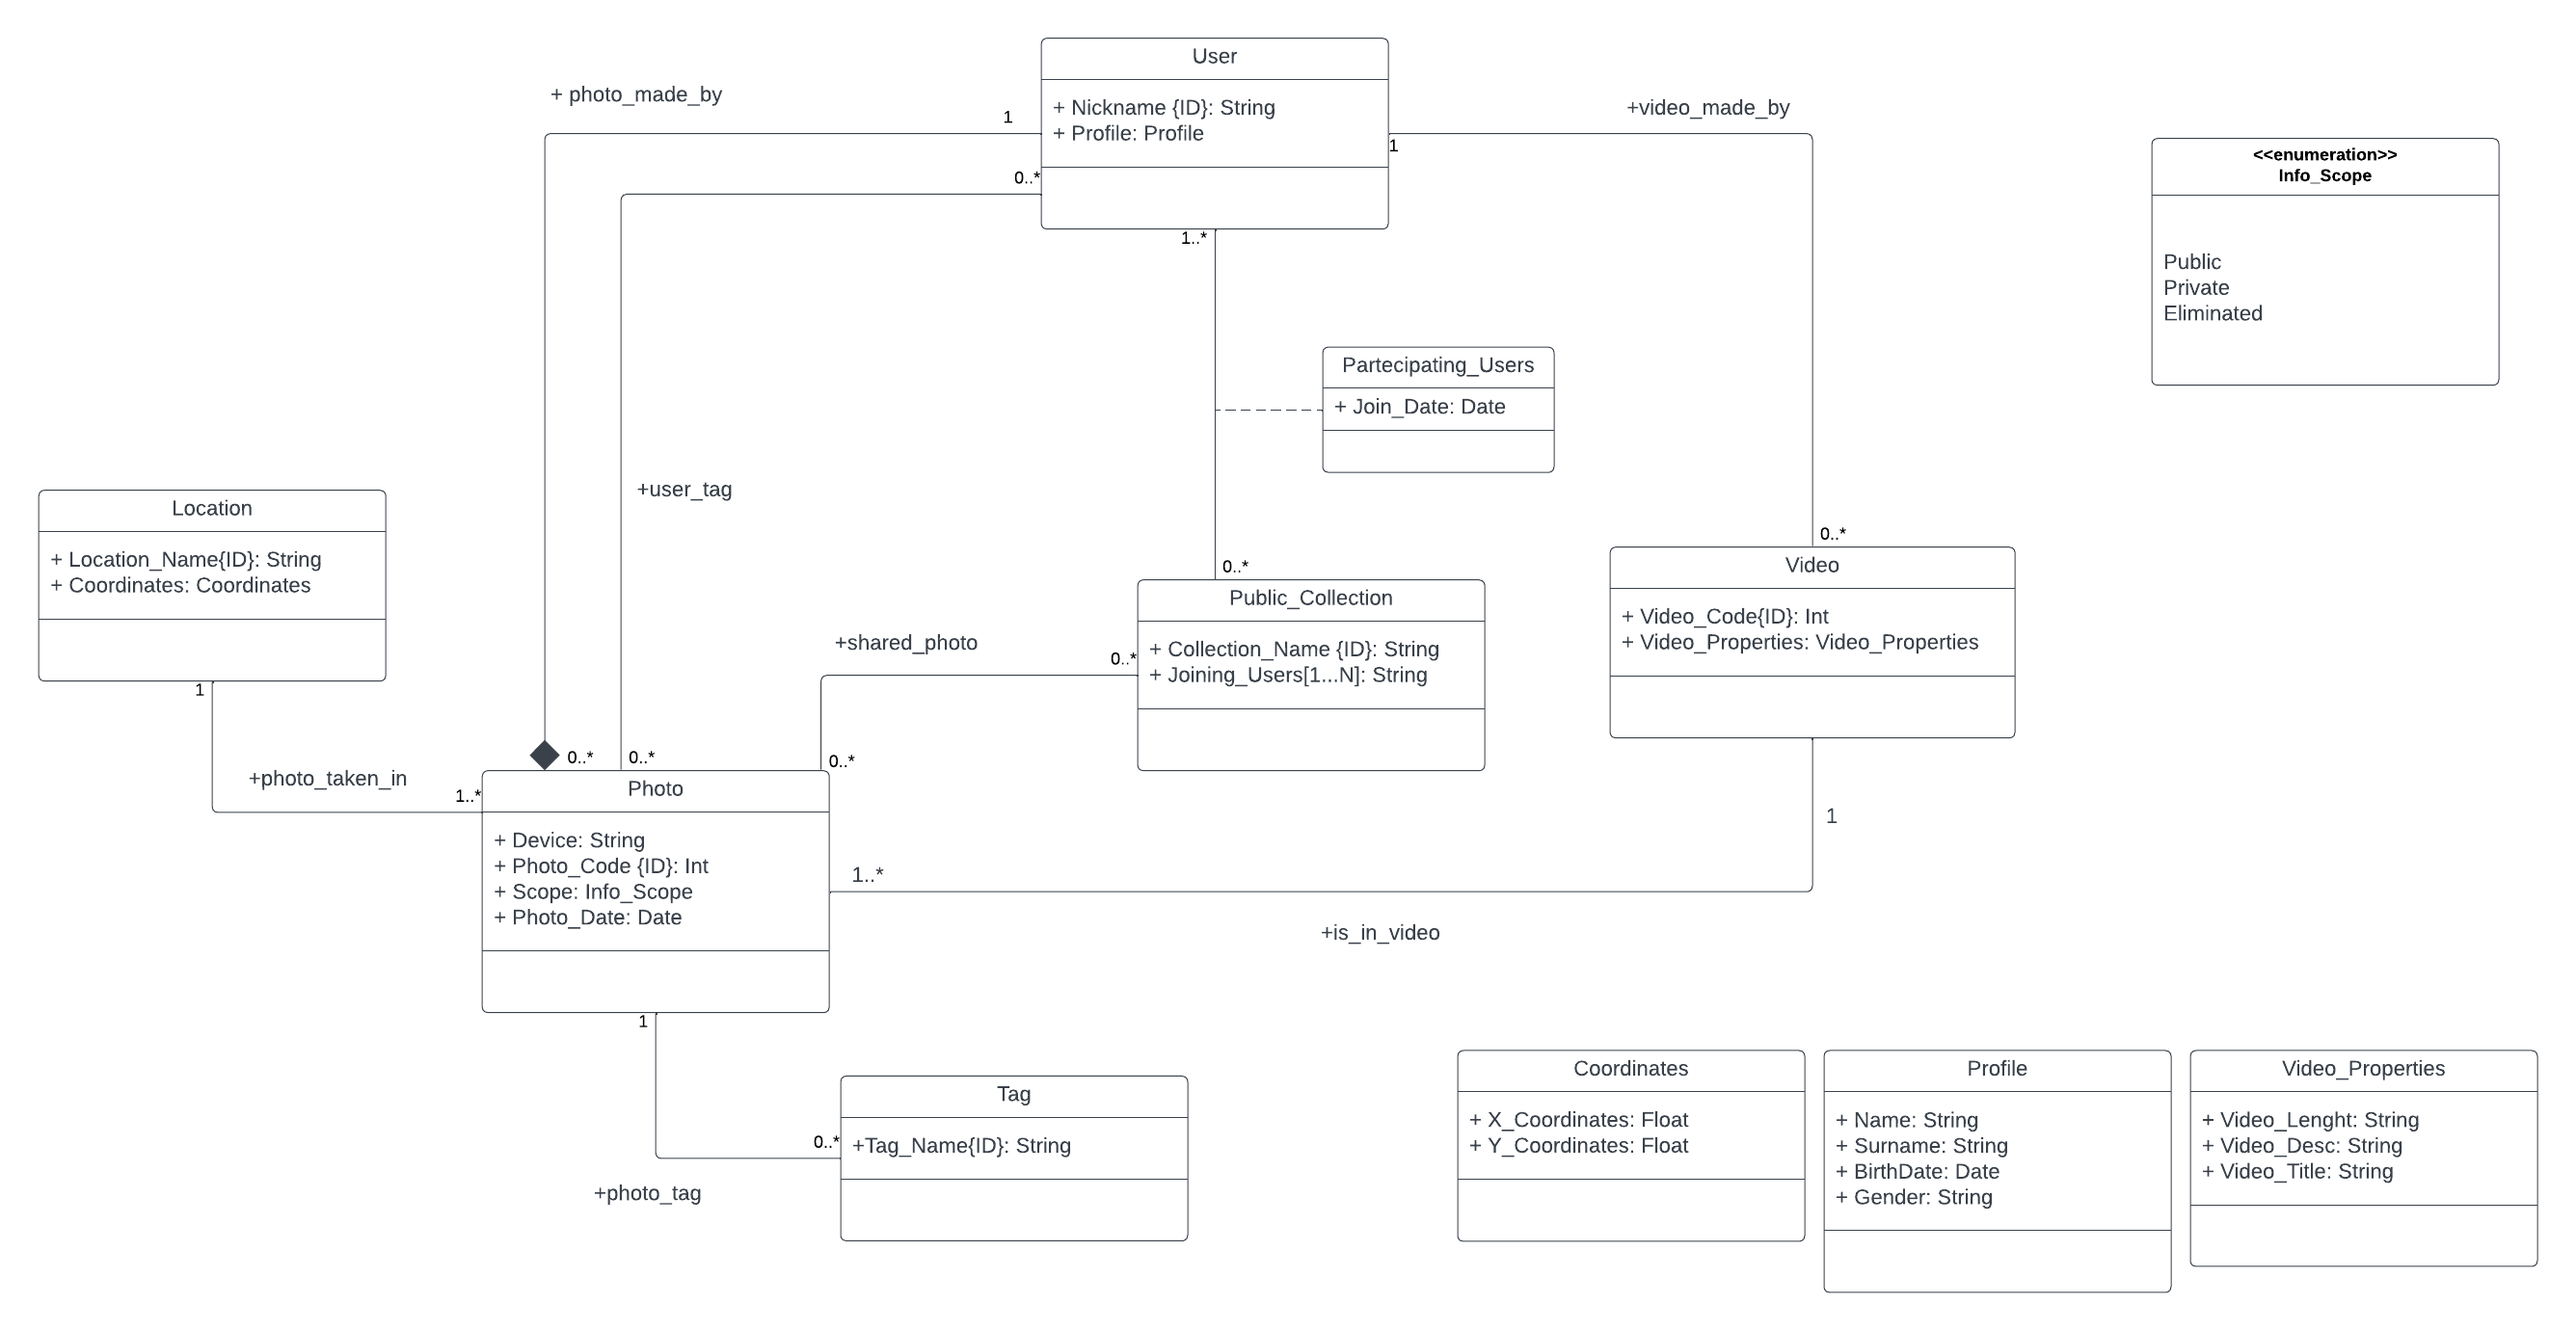
\includegraphics[width=1\linewidth]{Immagini/plogico1.png}
           \caption{Class Diagram in UML non ancora ristrutturato.}
        \end{figure}
    Dopo aver analizzato lo schema, passiamo quindi alla ristrutturazione del Class Diagram sopra illustrato, andando a definire nel dettaglio le motivazioni e le caratteristiche per ogni passaggio svolto.
        
        \subsection{Analisi delle ridondanze}

        Durante l'analisi delle ridondanze, è stato visto come, l'aggiunta di un attributo per il conteggio delle foto per luogo renda più efficiente le operazioni di recupero dei luoghi. Si è quindi presa la decisione di aggiungere l'attributo \textbf{"Photo Count"} in \textbf{"Location"}
            
        \subsection{Rimozione Generalizzazioni}

        Vista l'assenza di entità padri e figlie, non è stato necessario eliminare generalizzazioni.

        \subsection{Rimozione Attributi Multivalore}

        Nel modello non ristrutturato è presente un attributo multivalore, cioè \textbf{"Joining Users"}. 
        \break
        Nella ristrutturazione, è stato deciso di rimuovere completamente tale attributo, sfruttando invece l'associazione tra \textbf{"User"} e \textbf{"Public Collection"} per andare a tenere traccia degli utenti che partecipano a tale collezione.
            
        \subsection{Rimozione Attributi Strutturati}

        Nel modello non ristrutturato sono presenti più attributi strutturati, ovvero:
        \break\textbf{- "Coordinates"}
        \break\textbf{- "Profile"}
        \break\textbf{- "Video Properties"}
        \break
        Per ognuno di questi è stato deciso di estrarre tali attributi nelle rispettive entità.
            
        \subsection{Accorpamento/Partizionamento di Entità e Associazioni}
        Non è stato necessario svolgere operazioni di accorpamento o partizionamento.

        \pagebreak
        
        \subsection{Identificatore Chiavi Primarie}

        Sono stati scelti i seguenti attributi per assegnare le rispettive chiavi primarie:

        \vspace{1em}
      
        \begin{tabular}{|p{6cm}|p{5cm}|}
        \hline
        \textbf{Entità} & \textbf{Chiave Primaria}\\
        \hline
        User & Nickname \\
        \hline 
        Photo & Photo Code \\
        \hline 
        Location & Location Name \\
        \hline 
        Video & Video Code \\
        \hline 
        Public Collection & Collection Name \\
        \hline 
        Tag & Tag Name \\
        \hline 
        \end{tabular}

        \vspace{2em}
        
    \section{Class Diagram Ristrutturato}
        \subsection{Diagramma Ristrutturato}
        \begin{figure}[h]
            \centering
            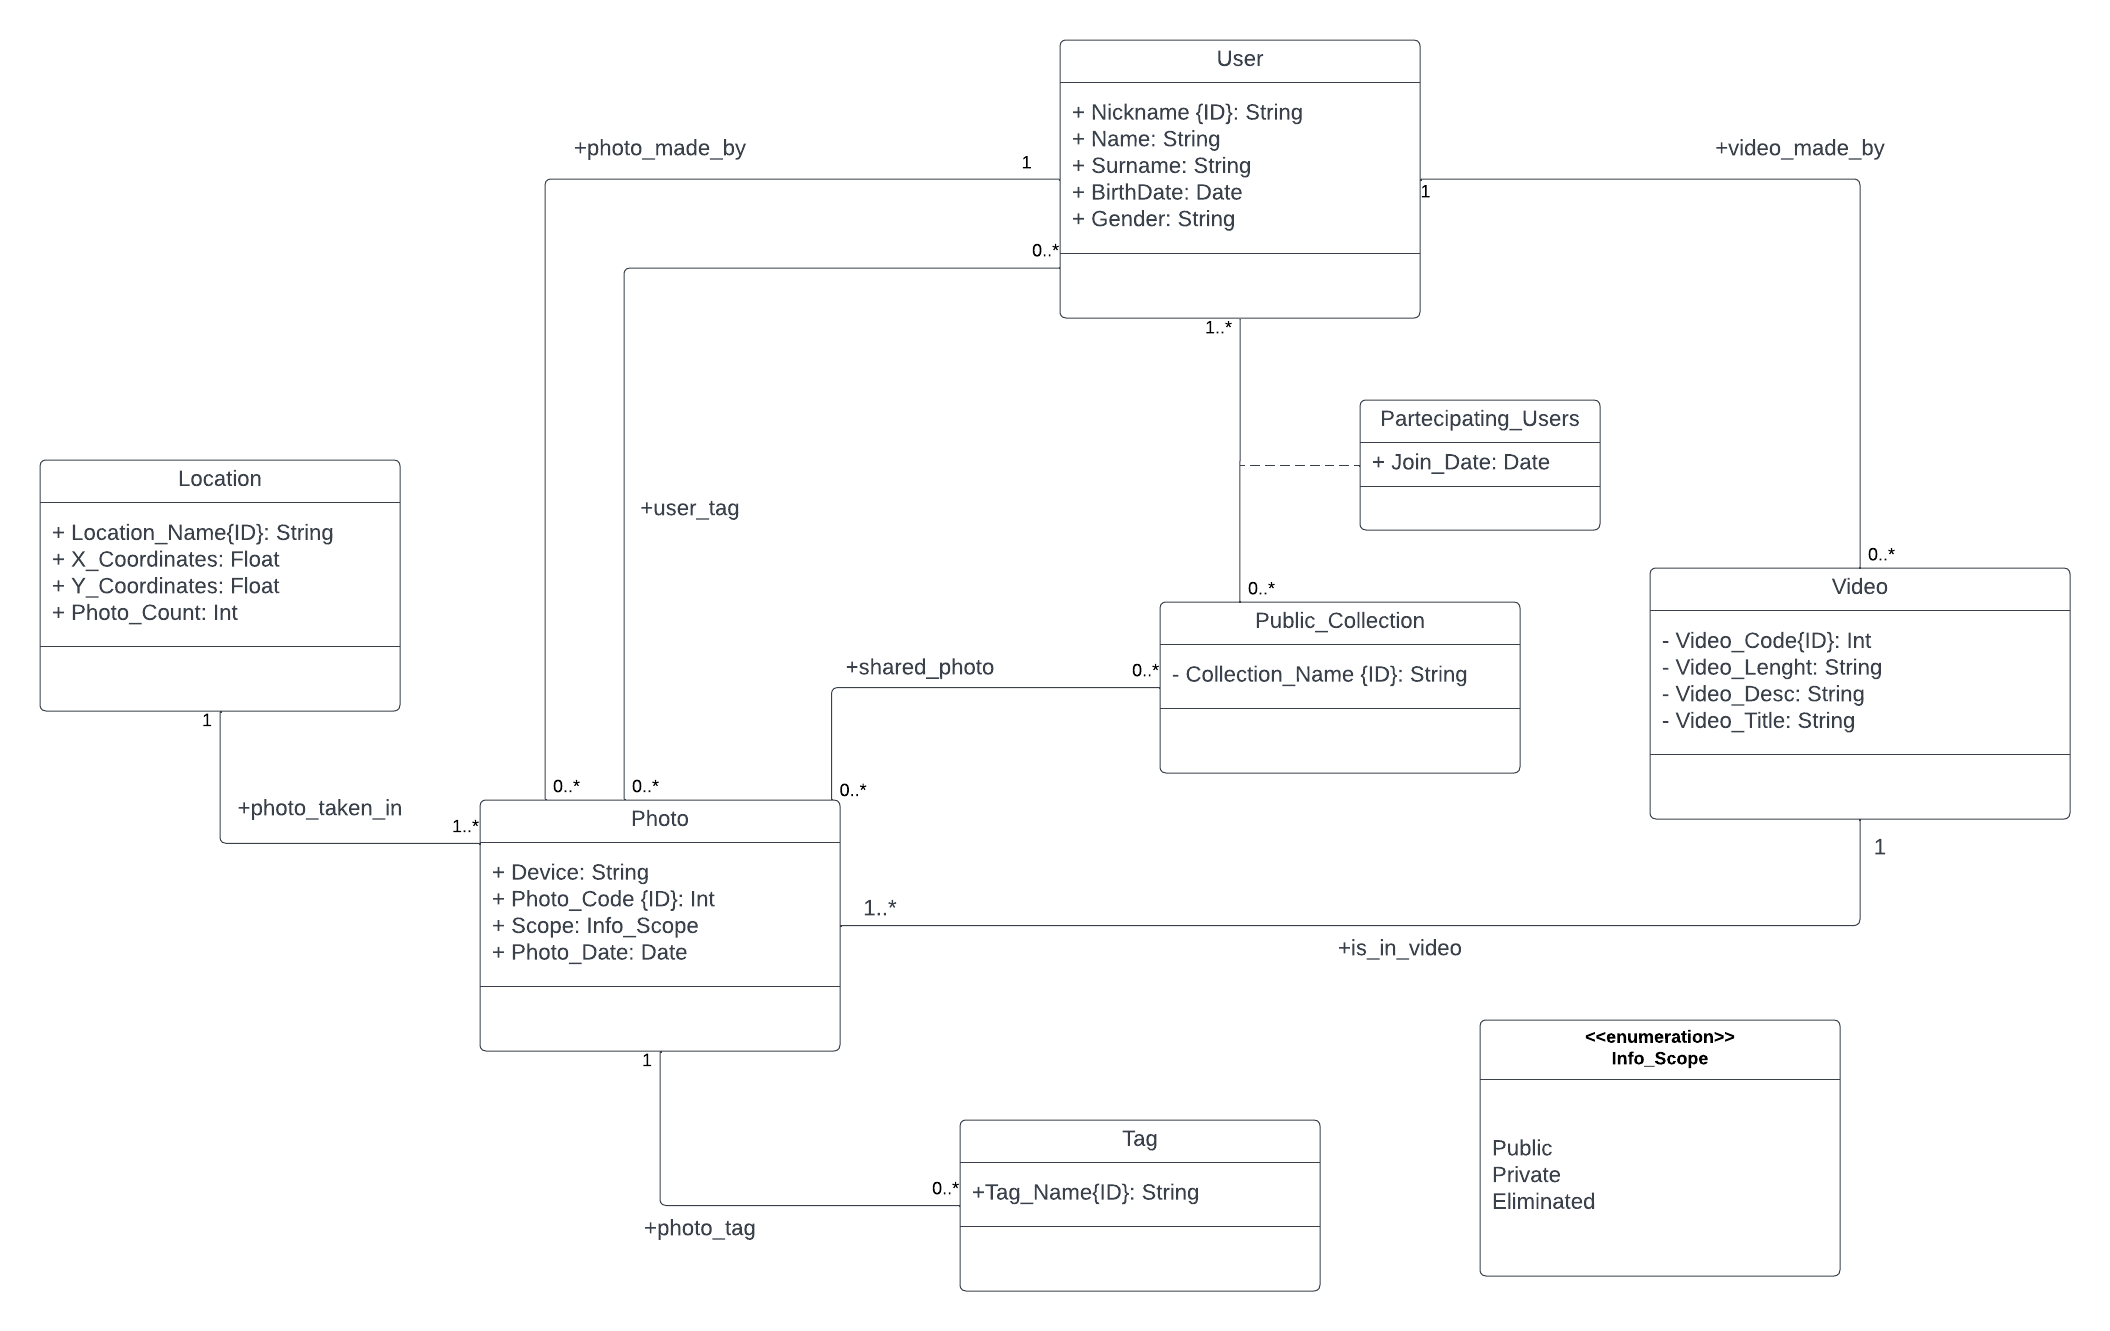
\includegraphics[width=1\linewidth]{Immagini/plogico2.png}
            \caption{Class Diagram in UML Ristrutturato.}
            \label{fig:galaxy}
        \end{figure}


